\documentclass[11pt]{article}
\usepackage[utf8]{inputenc}
\usepackage[margin=0.7in]{geometry}
\usepackage{amsmath,amssymb,enumitem,xcolor,multicol}
\usepackage[most]{tcolorbox}
\usepackage{pgfplots}\pgfplotsset{compat=1.17}
\setlength{\parindent}{0pt}
\definecolor{hookC}{HTML}{E8710A}
\definecolor{bigC}{HTML}{1A73E8}
\definecolor{vocabC}{HTML}{188038}
\definecolor{modelC}{HTML}{8430CE}
\definecolor{seeC}{HTML}{00897B}
\definecolor{wedoC}{HTML}{5F6368}
% one styled slide card; #1=color #2="Slide n" #3=heading
\newtcolorbox{slide}[3]{colback=#1!7,colframe=#1!75!black,coltitle=white,fonttitle=\bfseries,
  title={\small #2\hfill}\vspace{-2pt}\\[-2pt]{\large #3},breakable,boxrule=0.9pt,left=8pt,right=8pt,top=6pt,bottom=6pt,before skip=7pt,after skip=7pt}
\newcommand{\parthead}[1]{\vspace{6pt}{\color{bigC}\rule{\linewidth}{2pt}}\\[3pt]{\LARGE\bfseries\color{bigC!80!black} #1}\\[2pt]{\color{bigC}\rule{\linewidth}{2pt}}\vspace{6pt}}
\begin{document}

\begin{tcolorbox}[colback=bigC!85!black,colframe=bigC!85!black,coltext=white,boxrule=0pt,left=10pt,right=10pt]
{\LARGE\bfseries Algebra I --- Solving Quadratics by Factoring}\\[2pt]
{\normalsize Teacher Packet \textbullet\ Monday (Launch Day) \textbullet\ everything on one page to review}
\end{tcolorbox}

\parthead{Part 1 \; Slides (project these)}

\begin{slide}{hookC}{Slide 1 / 9 \textbullet\ Hook}{Why solve for zero?}
\begin{itemize}[leftmargin=1.3em,itemsep=1pt]
\item A ball's height is $h=-16t^{2}+64t$. When does it hit the ground?
\item That's a \textbf{quadratic} --- and we need to find WHEN $h=0$.
\item Graphing works but is slow --- there's a faster algebra trick this week.
\item By Friday you'll solve this in under 30 seconds.
\end{itemize}
\end{slide}

\begin{slide}{bigC}{Slide 2 / 9 \textbullet\ Big picture}{This week}
\begin{itemize}[leftmargin=1.3em,itemsep=1pt]
\item A quadratic can have $0$, $1$, or $2$ solutions (roots / zeros).
\item Factoring turns one hard equation into two easy ones.
\item \textbf{Key idea:} if two things multiply to $0$, one of them must BE $0$.
\item Mon $a{=}1$ \; Tue $a{\ne}1$ \; Wed/Thu special cases + mixed \; Fri quiz.
\end{itemize}
\end{slide}

\begin{slide}{vocabC}{Slide 3 / 9 \textbullet\ Vocabulary}{Today's terms}
\begin{itemize}[leftmargin=1.3em,itemsep=2pt]
\item \textbf{Quadratic equation:} form $ax^{2}+bx+c=0$.
\item \textbf{Root / zero / solution:} an $x$ that makes it true.
\item \textbf{Zero Product Property:} if $A\cdot B=0$ then $A=0$ or $B=0$.
\item \textbf{Factor:} rewrite as a product of simpler pieces.
\end{itemize}
\end{slide}

\begin{slide}{modelC}{Slide 4 / 9 \textbullet\ I do}{Model problem --- fully worked}
Solve $x^{2}+5x+6=0$.
\begin{itemize}[leftmargin=1.3em,itemsep=1pt]
\item Two numbers multiply to $6$, add to $5$ $\Rightarrow 2$ and $3$.
\item Factor: $(x+2)(x+3)=0$.
\item Zero Product Property: $x+2=0$ or $x+3=0$.
\item \textbf{Solutions:} $x=-2$ or $x=-3$ (check by substituting).
\end{itemize}
\end{slide}

\begin{slide}{seeC}{Slide 5 / 9 \textbullet\ See it}{The roots are where the parabola crosses the $x$-axis}
\begin{center}
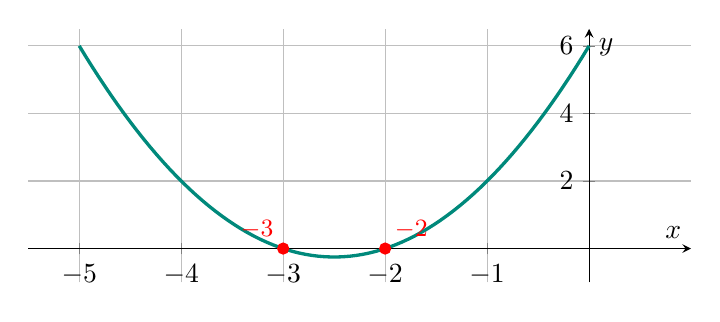
\begin{tikzpicture}
\begin{axis}[axis lines=middle,xlabel=$x$,ylabel=$y$,xmin=-5.5,xmax=1,ymin=-1,ymax=6.5,
 width=10cm,height=4.8cm,grid=both,xtick={-5,-4,-3,-2,-1,0},ytick={2,4,6},samples=80]
\addplot[very thick,seeC,domain=-5:0]{x^2+5*x+6};
\addplot[only marks,mark=*,red] coordinates {(-2,0)(-3,0)};
\node[above left,red,font=\small] at (axis cs:-3,0){$-3$};
\node[above right,red,font=\small] at (axis cs:-2,0){$-2$};
\end{axis}
\end{tikzpicture}
\end{center}
$y=x^{2}+5x+6$ crosses at $x=-3$ and $x=-2$ --- the same answers we factored.
\end{slide}

\begin{slide}{wedoC}{Slide 6 / 9 \textbullet\ We do \#1}{Together --- whiteboards up}
Solve $x^{2}+7x+10=0$. \hfill \textcolor{modelC}{$(x+2)(x+5)=0\Rightarrow x=-2,\,-5$}
\end{slide}

\begin{slide}{wedoC}{Slide 7 / 9 \textbullet\ We do \#2}{Different signs --- think carefully}
Solve $x^{2}-2x-15=0$. \hfill \textcolor{modelC}{$(x-5)(x+3)=0\Rightarrow x=5,\,-3$}
\end{slide}

\begin{slide}{wedoC}{Slide 8 / 9 \textbullet\ We do \#3}{No middle term --- special case}
Solve $x^{2}-9=0$ (difference of squares). \hfill \textcolor{modelC}{$(x-3)(x+3)=0\Rightarrow x=3,\,-3$}
\end{slide}

\begin{slide}{bigC}{Slide 9 / 9 \textbullet\ Roadmap}{Where we're going}
\begin{itemize}[leftmargin=1.3em,itemsep=1pt]
\item \textbf{Today:} factor when $a=1$, Zero Product Property.
\item \textbf{Tue:} factor when $a\ne 1$ (e.g.\ $2x^{2}+7x+3$).
\item \textbf{Wed/Thu:} special cases + mixed practice. \quad \textbf{Fri:} quiz.
\end{itemize}
\end{slide}

\parthead{Part 2 \; Group examples --- worked for you}
\begin{enumerate}[leftmargin=1.6em,itemsep=4pt]
\item $x^{2}+7x+10=0$:\ product $10$, sum $7\to 2,5$; $(x+2)(x+5)=0$; $x=-2,-5$.
\item $x^{2}-2x-15=0$:\ product $-15$, sum $-2\to -5,3$; $(x-5)(x+3)=0$; $x=5,-3$.
\item $x^{2}-9=0$:\ difference of squares; $(x-3)(x+3)=0$; $x=3,-3$.
\end{enumerate}

\parthead{Part 3 \; Guided notes (teacher key --- blue = answers)}
\textbf{Vocabulary}\\[3pt]
\textbf{Zero Product Property:} if $A\cdot B=\textcolor{blue!65!black}{\underline{0}}$, then $A=\textcolor{blue!65!black}{\underline{0}}$ or $B=\textcolor{blue!65!black}{\underline{0}}$.\\[6pt]
\textbf{Root (solution):} an $x$ that makes the equation \textcolor{blue!65!black}{\underline{true}}; on a graph it is an \textcolor{blue!65!black}{\underline{$x$-intercept}}.\\[8pt]
\textbf{We do together.}\quad Solve $x^{2}+5x+6=0$.
\begin{enumerate}[label=\textbf{Step \arabic*.},leftmargin=3em,itemsep=3pt]
\item One side already $=0$. Good.
\item Factor: $x^{2}+5x+6=\big(\textcolor{blue!65!black}{\underline{x+2}}\big)\big(\textcolor{blue!65!black}{\underline{x+3}}\big)$.
\item Set each factor $=0$: \ $\textcolor{blue!65!black}{\underline{x+2}}=0$ \ or \ $\textcolor{blue!65!black}{\underline{x+3}}=0$.
\item Solve: \ $x=\textcolor{blue!65!black}{\underline{-2}}$ \ or \ $x=\textcolor{blue!65!black}{\underline{-3}}$.
\end{enumerate}
\vspace{2pt}\textbf{You Try:} a) $x^{2}-x-12=0$ \ \textcolor{blue!65!black}{$(x-4)(x+3)=0\Rightarrow x=4,-3$}; \ b) $x^{2}-9=0$ \ \textcolor{blue!65!black}{$(x-3)(x+3)=0\Rightarrow x=3,-3$}.

\parthead{Part 4 \; Worksheet (student copy)}
\fbox{\parbox{0.97\linewidth}{\small\textbf{Final answers} (show your work):\\[5pt]1.~\underline{\hspace{1.2cm}}\ 2.~\underline{\hspace{1.2cm}}\ 3.~\underline{\hspace{1.2cm}}\ 4.~\underline{\hspace{1.2cm}}\ 5.~\underline{\hspace{1.2cm}}\ 6.~\underline{\hspace{1.2cm}}\ 7.~\underline{\hspace{1.2cm}}\ 8.~\underline{\hspace{1.2cm}}\ 9.~\underline{\hspace{1.2cm}}\ 10.~\underline{\hspace{1.2cm}}\ 11.~\underline{\hspace{1.2cm}}}}
\vspace{6pt}
\textbf{Directions: Solve each by factoring. State both roots.}
\begin{multicols}{2}
\begin{enumerate}[label=\textbf{\arabic*.},itemsep=1.1cm]
\item $x^{2}+5x+6=0$
\item $x^{2}+7x+10=0$
\item $x^{2}-2x-15=0$
\item $x^{2}-9=0$
\item $x^{2}+8x+16=0$
\item $x^{2}-6x+8=0$
\item $x^{2}+x-12=0$
\item $x^{2}-25=0$
\item $x^{2}-4x=0$
\item $x^{2}+2x-8=0$
\end{enumerate}
\end{multicols}
\vspace{2pt}\hrule\vspace{4pt}\textbf{Challenge} (preview of $a\ne1$):
\begin{enumerate}[label=\textbf{\arabic*.},start=11,leftmargin=1.6em]
\item $2x^{2}+5x-3=0$
\end{enumerate}

\parthead{Part 5 \; Answer key --- fully worked}
\textbf{Procedure:} make one side $=0$, factor, set each factor to $0$, solve.\\[6pt]
\begin{enumerate}[label=\textbf{\arabic*.},itemsep=3pt]
\item $(x+2)(x+3)=0\Rightarrow x=-2,\,-3$
\item $(x+2)(x+5)=0\Rightarrow x=-2,\,-5$
\item $(x-5)(x+3)=0\Rightarrow x=5,\,-3$
\item $(x-3)(x+3)=0\Rightarrow x=3,\,-3$
\item $(x+4)^{2}=0\Rightarrow x=-4$ (double root)
\item $(x-2)(x-4)=0\Rightarrow x=2,\,4$
\item $(x+4)(x-3)=0\Rightarrow x=-4,\,3$
\item $(x-5)(x+5)=0\Rightarrow x=5,\,-5$
\item $x(x-4)=0\Rightarrow x=0,\,4$
\item $(x+4)(x-2)=0\Rightarrow x=-4,\,2$
\item $2x^{2}+5x-3=(2x-1)(x+3)=0\Rightarrow x=\tfrac{1}{2},\,-3$
\end{enumerate}
\end{document}
